\section{Broadcast: Delivery Without Acknowledgment}
\label{sec:broadcast}

Speech and telemetry cannot wait for a retransmission, so they need a
mode in which nothing is repeated and the receiver's only contribution
is a report that it was heard.  This section has two halves.  The
first (\S\ref{sec:broadcast}--\S\ref{sec:bcreport}) is the design and
its measurement on the simulated channels: the frame format, what an
exchange looks like, the group-size question under fading, and a
listener report that was measured and rejected.  The second
(\S\ref{sec:cport_bcast}) is what the boards then required of it ---
a fourth receive path, a rung policy, a chunked file source, and a
sender-signalled statistics exchange that supplies the feedback the
first half had left as future work.  The transport for this already
exists:
a broadcast is a streamed burst (Section~\ref{sec:stream}) with the
acknowledgment machinery subtracted --- no acknowledgment request, no
window, no selective repeat, no reply timer.  What has to be added is
the one thing a burst does not need.  A burst has exactly one listener,
who was already there; a broadcast must let a receiver that tunes in
mid-transmission join.  Every group therefore re-sends the preamble and
opens with a \textsc{sync} frame carrying the stream descriptor, so a
late listener acquires at the next group boundary rather than waiting
for the broadcast to end.

Framing is two bytes per frame: a \textsc{sync} bit, an \textsc{eos}
bit, a six-bit sequence number used \emph{only} for loss statistics, and
the count of valid payload bytes in that frame.  The obvious model to
copy would be RTP, and copying it would be a mistake: its twelve-byte
fixed header is 91\,ms of air time at the top rung, so a
20\,ms-packetised stream would carry 1.75 bytes of payload behind
12 bytes of header.  What survives the transplant is what a receiver
cannot work out for itself --- sequence, stream boundaries and payload
type.  What does not is the timestamp (this link's delay is
deterministic, so a frame's position in the stream \emph{is} its
timestamp), the synchronisation source identifier, and the per-packet
payload type, which rides the \textsc{sync} frame instead.

Carrying the length in \emph{every} frame rather than only in the
\textsc{eos} frame costs about 4\,\% at 26-byte frames and buys a
property that only matters when nothing is retransmitted: every frame
is self-delimiting, so losing the one frame that would have carried the
length does not mis-size the payload.

The rate ladder decides what can be carried at all.  Codec2 at
700\,bit/s fits only rungs 11--12 (941 and 1\,059\,bit/s user rate,
$+2.6$ and $+4.7$\,dB); Codec2 450 fits rungs 8--9; below rung 8 this
mode carries telemetry only, down to EXTREME's 7.8\,bit/s.  That
envelope is set by the waveform, not by the protocol above it.

\begin{table}[H]
    \centering
    \caption{Broadcast delivery, 200-byte payload in groups of four
             (\texttt{experiments/broadcast\_demo.py}, 20 trials per
             point).  Nothing is retransmitted, so ``recovered'' is
             payload bytes reassembled against bytes sent.}
    \label{tab:broadcast}
    \begin{tabular}{lccc}
        \toprule
        & all recovered & $\ge$90\,\% & breaks down \\
        \midrule
        speech, rung 12 (16-QAM 3/4)  & $+9.5$\,dB & $+5.0$\,dB & $+2$\,dB \\
        telemetry, rung 7 (QPSK 1/2)  & $+1.5$\,dB & $-3.0$\,dB & $-6$\,dB \\
        \bottomrule
    \end{tabular}
\end{table}

\begin{figure}[H]
    \centering
    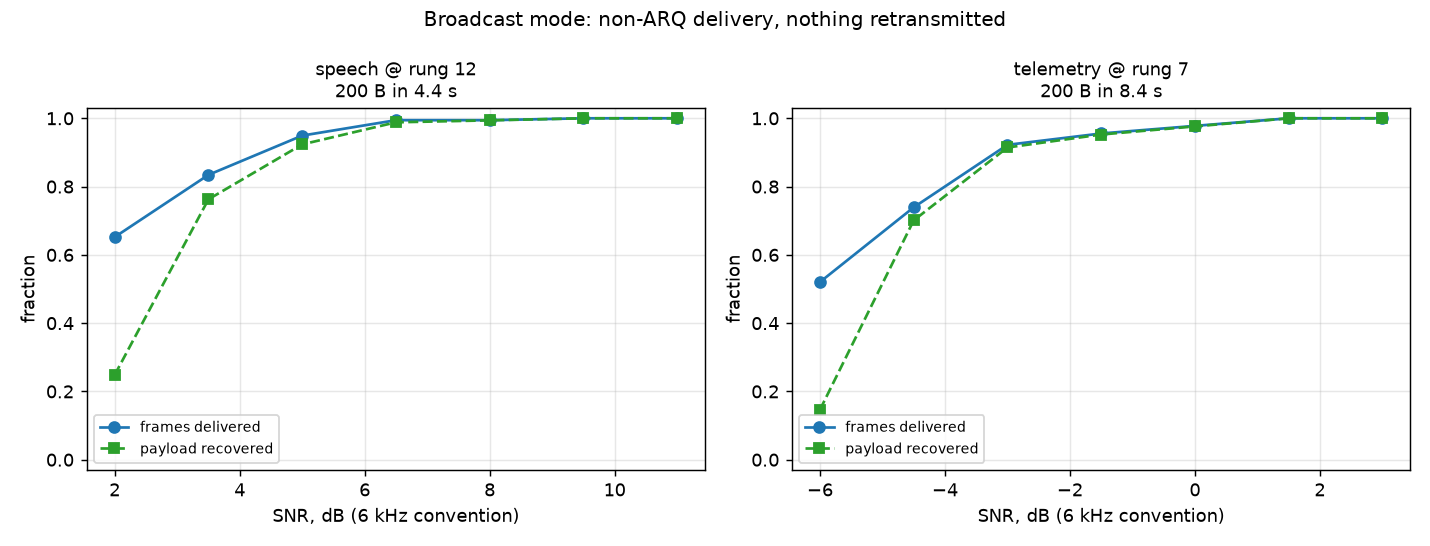
\includegraphics[width=\textwidth]{images/broadcast_demo.png}
    \caption{Non-ARQ delivery against SNR.  Frames delivered runs above
             payload recovered at the low end because a frame lost from
             the middle of a group costs its own bytes while still
             being counted in the span.}
    \label{fig:broadcast}
\end{figure}

\subsection{What a Broadcast Exchange Actually Looks Like}
\label{sec:broadcast_seq}

Figure~\ref{fig:bcseq} traces a 14162-byte file broadcast over the
virtual channel.  Three properties of the sequence are worth drawing
out, because each was established by a failure rather than by design.

\emph{The rung is fixed at engage.}  A broadcast cannot renegotiate
within a group, so it runs at whatever the link last established ---
and the link must be established first: below rung~4 a broadcast cannot
be carried at all, so the sender probes with a control frame and waits
rather than refusing outright.  (Two later refinements keep this
property but move the decision: the firmware's hold-and-probe of
\S\ref{sec:cport_bcast} makes the wait explicit and bounded, and the
block statistics of \S\ref{sec:bcstats} let the rung change
\emph{between} blocks, since every group re-announces its geometry.)

\emph{The listener stays silent.}  On a simplex channel, transmitting
is precisely what stops a station hearing, and a broadcast is a train
of transmissions with gaps of well under a second between turns.  Those
gaps read as an idle channel to carrier sense, so a station holding a
pending reply fires into one and is deaf as the next transmission's
preamble goes past.  Losing a group's preamble costs the entire group:
measured, a single 0.8\,s reply cost exactly 16 frames on a $+20$\,dB
channel.  A station that is hearing a broadcast therefore treats the
channel as busy, which suppresses the transmission \emph{and} stops
the link layer scoring the resulting reply timeouts as losses.

\emph{\textsc{eos} ends the walk, not the group descriptor.}  The final
group of a broadcast is normally short, but the descriptor can only
advertise the nominal size --- it carries $\log_2$ of the group.  A
receiver that trusts the descriptor walks blocks that were never
transmitted, and while stepping through blocks it is not running the
preamble detector: 15 phantom CRC failures, each costing a block-time
of deafness.  The \textsc{eos} bit is the stop signal, with a
consecutive-failure bound for the case where the \textsc{eos} frame is
itself lost.

\begin{figure}[H]
    \centering
    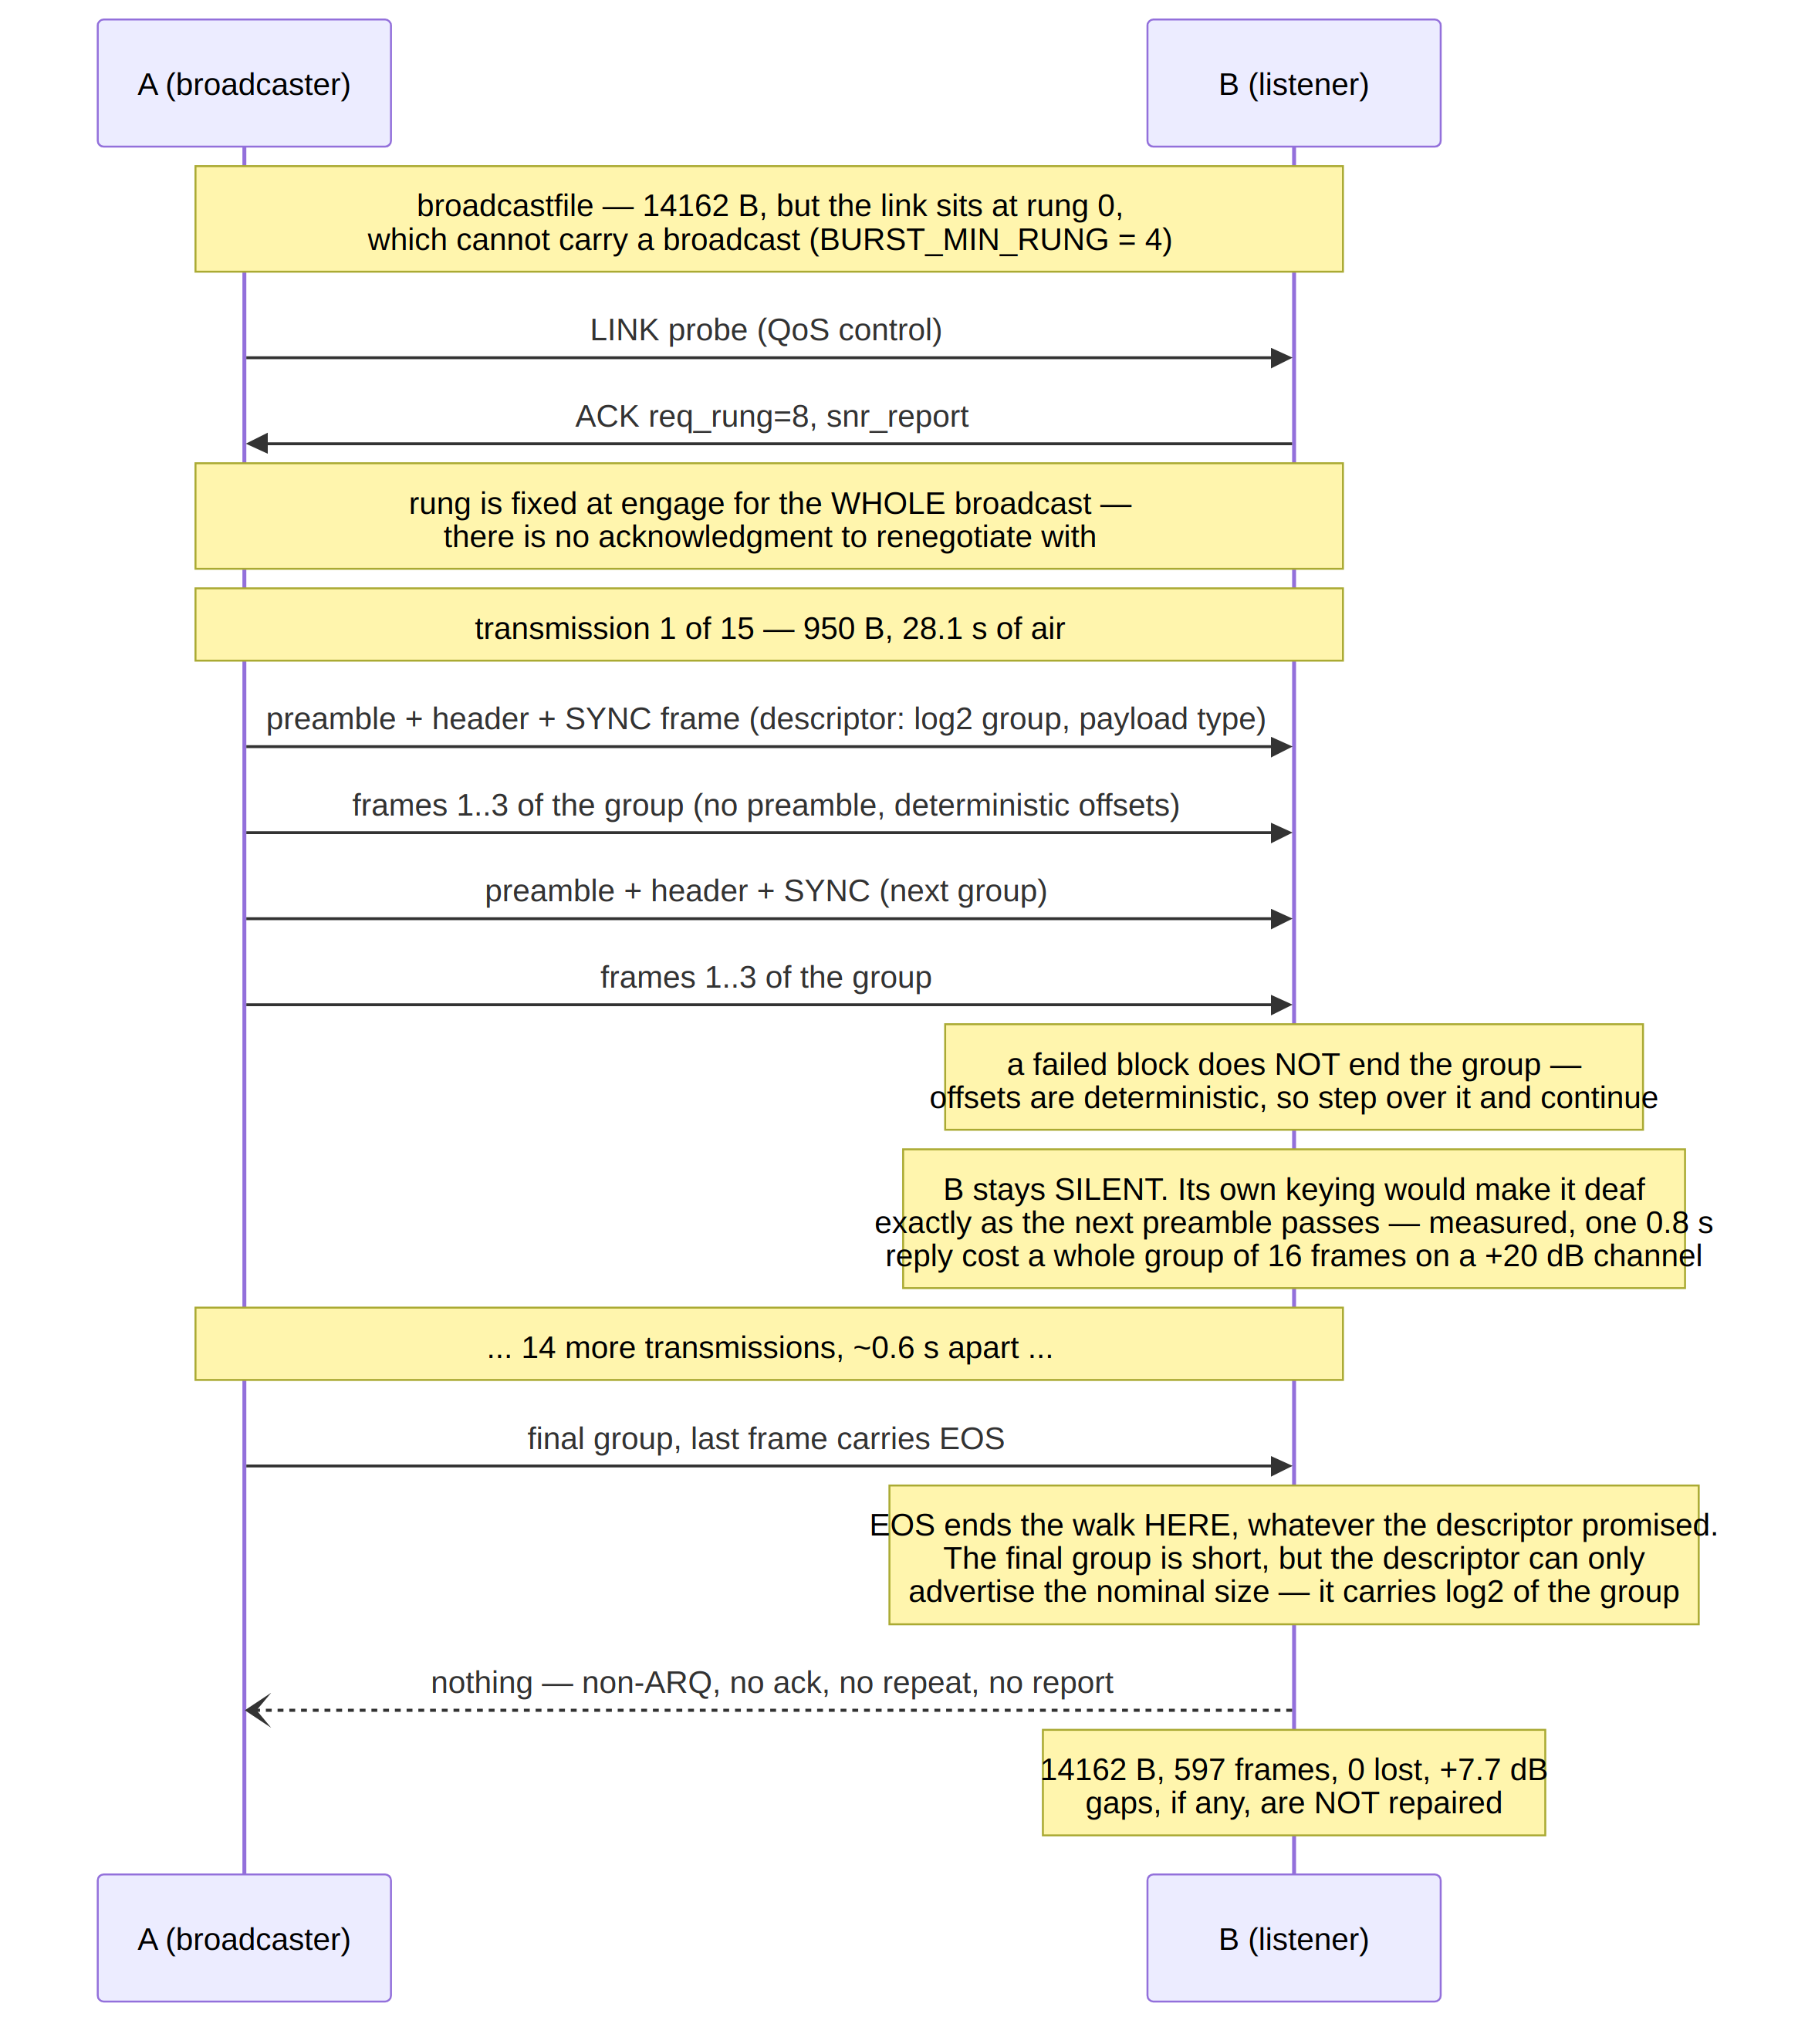
\includegraphics[width=0.95\textwidth]{images/broadcast_seq.png}
    \caption{A file broadcast: link probe, then transmissions carrying
             one preamble per group, with no acknowledgment of any kind
             in return.  The listener's silence is a protocol
             requirement, not an omission.}
    \label{fig:bcseq}
\end{figure}

\subsection{Group Size Under Fading}
\label{sec:bcgroup}

Group size is the one free parameter of the mode, and on a clean
channel it looks free in both directions: a 14162-byte file arrives
complete and byte-identical at groups of 4, 8 and 16 alike.  That
result says nothing, because it exercises only half of the trade.  One
preamble amortised over more frames is the benefit; the cost is that a
missed acquisition takes the whole group with it, and a broadcast
retransmits nothing.  The cost term only fires when acquisitions are
actually missed, which on a clean channel they are not.

Figure~\ref{fig:bcfading} runs the same three group sizes against SNR
with Rayleigh fading enabled (0.5\,Hz, roughly a 2\,s fade period),
30 trials per point, all three sizes facing the same fading realisation
at each point so the comparison is paired rather than three independent
samples of a noisy quantity.

The left panel is the metric that matters, and it is flat: mean payload
recovery is 64.4\,\%, 62.5\,\% and 62.3\,\% for groups of 4, 8 and 16.
The spread between them is smaller than the point-to-point scatter, so
on this evidence a larger group buys nothing.

The right panel is where the trade becomes visible.  Frames
\emph{decoded} does rise with group size --- there are fewer preambles
to miss --- but payload recovered does not follow it, and the gap
between the two is the payload lost behind a missed acquisition.  That
gap is monotonic in group size and well outside the scatter: 4.8,
8.6 and 15.5 points on average.  A group of 16 at $+2$\,dB decodes
89.3\,\% of frames while recovering 65.0\,\% of the payload.

The practical reading is that group size trades \emph{granularity} of
loss, not quantity.  Above $+5$\,dB all three are equivalent and the
larger group is free: with the same 0.5\,Hz fading and a $+20$\,dB
nominal channel, the 14162-byte file still arrived complete and
byte-identical at a group of 8, the fading having pulled the measured
SNR to $+2.4$\,dB and the link down one rung.  Below that the larger
group concentrates the same loss into fewer, longer holes.  For
telemetry reassembled whole this is strictly worse; for speech, where
one long dropout is more objectionable than several short ones, worse
again.

The demonstration application caps the group at 8, which is the ceiling
its static receive buffer imposes rather than a value this figure
argues for --- on these measurements 4 is the better default whenever
fading is expected, and the choice should follow the channel rather
than the buffer.  The firmware caps it by \emph{air time} instead
(\S\ref{sec:cport_bcast}): four frames per group at rung~4 and one at
EXTREME, so that a keying never outlasts the carrier-sense time
constants.

\begin{figure}[H]
    \centering
    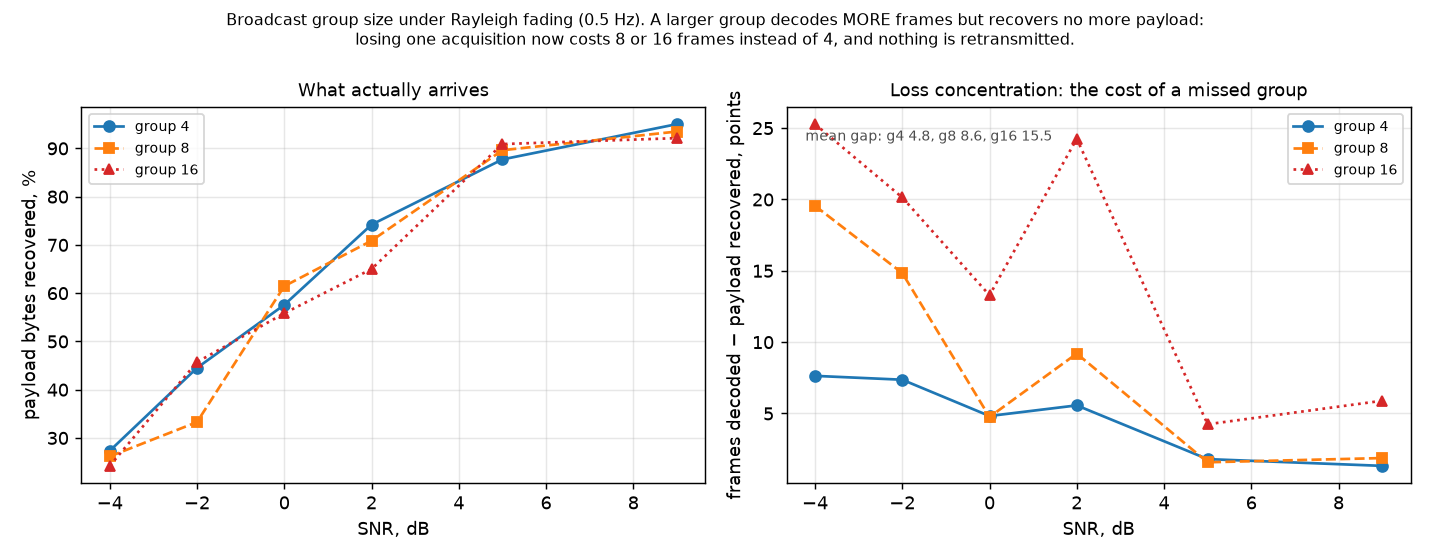
\includegraphics[width=\textwidth]{images/broadcast_fading.png}
    \caption{Broadcast group size under 0.5\,Hz Rayleigh fading
             (\texttt{experiments/broadcast\_fading.py}, 30 trials per
             point, paired realisations).  Payload recovery is
             indistinguishable across group sizes; what changes is how
             the loss is distributed.}
    \label{fig:bcfading}
\end{figure}

\subsection{A Reception Report: Measured and Rejected}
\label{sec:bcreport}

The gap this leaves is real.  A 14162-byte broadcast ran its entire
450\,s at rung~8 while the listener was decoding it at $+7.7$\,dB ---
enough for rung~12, which would have cut each turn from 28.1\,s to
5.1\,s.  Worse, broadcast frames deliberately never reach the ARQ
path, so during a broadcast \emph{neither} station's controller sees
traffic and the staleness decay walks both ladders down: after 454\,s
of broadcasting, the next file transfer opened at rung~4 and spent
37.0\,s on a frame that rung~12 delivers in 5.1\,s.

A listener report was therefore implemented, in a quiet window left by
the sender, and then removed.  Table~\ref{tab:bcreport} is why.

\begin{table}[H]
    \centering
    \caption{Listener reception reports, 14162-byte broadcast,
             597 frames sent, $+20$\,dB channel.  The mode repairs
             nothing, so every lost frame is lost for good.}
    \label{tab:bcreport}
    \begin{tabular}{lccc}
        \toprule
        & frames lost & turns & rung \\
        \midrule
        no report (run 1)    & 0  & 15 & 8 fixed \\
        no report (run 2)    & 4  & 15 & 8 fixed \\
        report per group     & 32 & 10 & $8\rightarrow11$ \\
        report per turn      & 28 & 16 & $8\rightarrow7$ \\
        \bottomrule
    \end{tabular}
\end{table}

Rate-limiting the report to one per turn removed the storm and bought
nothing: the same turn count, 28 frames lost permanently, and the rung
moved \emph{down}.  The feedback is self-defeating in a way tuning
cannot fix --- the listener's own transmission causes losses, the
losses make the controller conservative, and the broadcast gets slower.
The root cause is that the listener infers ``the sender has paused''
from quiet on its own clock, while it decodes \emph{behind} the sender
(lag of seconds; 11.7\,s was measured on a 16-block group), so its
reply lands inside the next transmission whatever threshold is chosen,
and a window wide enough to absorb the lag costs more air than the rung
climb saves.

Doing this properly requires the \emph{sender} to signal an explicit
report slot on the wire, so the listener answers a marker instead of
inferred silence.  It was left as future work at this point and then
built on the boards, where it was needed: the end-of-block marker and
statistics reply of \S\ref{sec:bcstats} are exactly this mechanism,
and the fading harness of \S\ref{sec:bcfade} is where its control laws
were proven.  The rejected listener-side report above is why the
marker had to come from the sender.

Telemetry reaches 90\,\% delivery at $\approx-3.1$\,dB against rung 7's
$-5.3$\,dB acknowledged-mode sensitivity.  That $\approx$2\,dB is the
honest price of non-ARQ: a frame that fails is simply gone, and a group
whose preamble is missed takes four frames with it.  A receiver that
tuned in half-way through the first group of seven recovered 90\,\% of
the remainder --- it cannot, of course, recover what it never heard.

Two findings from building this generalise beyond broadcast.

The first concerns the detector.  \texttt{detect\_preamble} takes a
\emph{global} argmax over whatever slice it is handed, so a slice
containing several groups makes it lock the strongest preamble rather
than the first, and every group before that one is silently lost --- 300
samples of lead-in were enough to skip a whole group.  The slice must
therefore be bounded on \emph{both} sides so that it holds exactly one
preamble.  Starting the slice on a preamble is not sufficient; nor can
the far edge be found by searching forward for the next preamble, since
from inside a group the detector false-locks on data.  The bound is
geometry --- preamble plus header plus blocks --- and because the first
decode necessarily runs before that geometry is known, the receiver
learns the extent from it and then restarts the walk with the bound in
place.  Anything that scans a recording containing multiple frames has
the same exposure.

The second concerns LLR calibration (Section~\ref{sec:llr}), which
matters more here than under ARQ for a simple reason: a frame the
decoder cannot recover is not retried, it is lost.  Enabling the
measured reliability map moved telemetry from 30.6\,\% to 69.8\,\% of
payload recovered at $-4.5$\,dB and from 3.4\,\% to 12.0\,\% at
$-6$\,dB, while changing nothing above $-3$\,dB where delivery is
already near perfect.  It is therefore on by default in this mode.  The
map is gated to $\mu \le 2$ because it was trained on BPSK/QPSK
statistics, and the speech column of the sweep came back
\emph{bit-identical} with the map enabled --- an incidental but clean
confirmation that the gate does what it claims.

What broadcast gives up is the feedback path.  The rate-adaptation
mechanisms of Section~\ref{sec:link} all depend on the peer replying,
and here it does not.  Either the sender schedules periodic listening
gaps in which receivers return the statistics above, at the cost of the
continuous transmission that makes broadcast cheap, or it does not
adapt at all: announce a rung in the descriptor and hold it.
STANAG~5066's non-ARQ delivery mode takes the second course, and it
remains the default here for a broadcast to \emph{strangers} --- a
broadcast has no single listener to adapt to.  When the sender holds a
capability record for the peer that declares it will answer, the
firmware takes the first course, with blocks of about 45\,s and a
reply window sized to the exchange (\S\ref{sec:bcstats}); measured
under a fade, that adaptation delivers 32--39\,\% more of the stream
than a held rung (\S\ref{sec:bcfade}).

\subsection{Broadcast on the Boards}
\label{sec:cport_bcast}

Broadcast (Section~\ref{sec:broadcast}) is delivery without
acknowledgment: a streamed burst with the ARQ machinery subtracted,
plus a SYNC frame at the head of every group so a receiver that was not
there at the start can join. Both models implement it as a
\emph{recording} walk --- \texttt{bc\_receive()} takes a slice of audio
and scans it for groups --- and that is exactly what a board cannot do.
The firmware never holds a recording: samples arrive 256 at a time out
of a capture FIFO and leave through a streaming receiver that emits one
event per decoded (or failed) block.

So the boards needed a fourth path. \texttt{usb\_radio\_main.c} builds
one group per keying and walks the received group with
\texttt{bc\_advance()} over that streaming receiver --- the same
\texttt{rxs\_continue\_burst()} stepping burst ARQ uses
(Section~\ref{sec:cport_burstdebug}), with the acknowledgment machinery
absent rather than removed. Figure~\ref{fig:bcastboards} traces one
broadcast across the wire. Three properties had to be right that no
host model ever faced.

\begin{figure}[htbp]
    \centering
    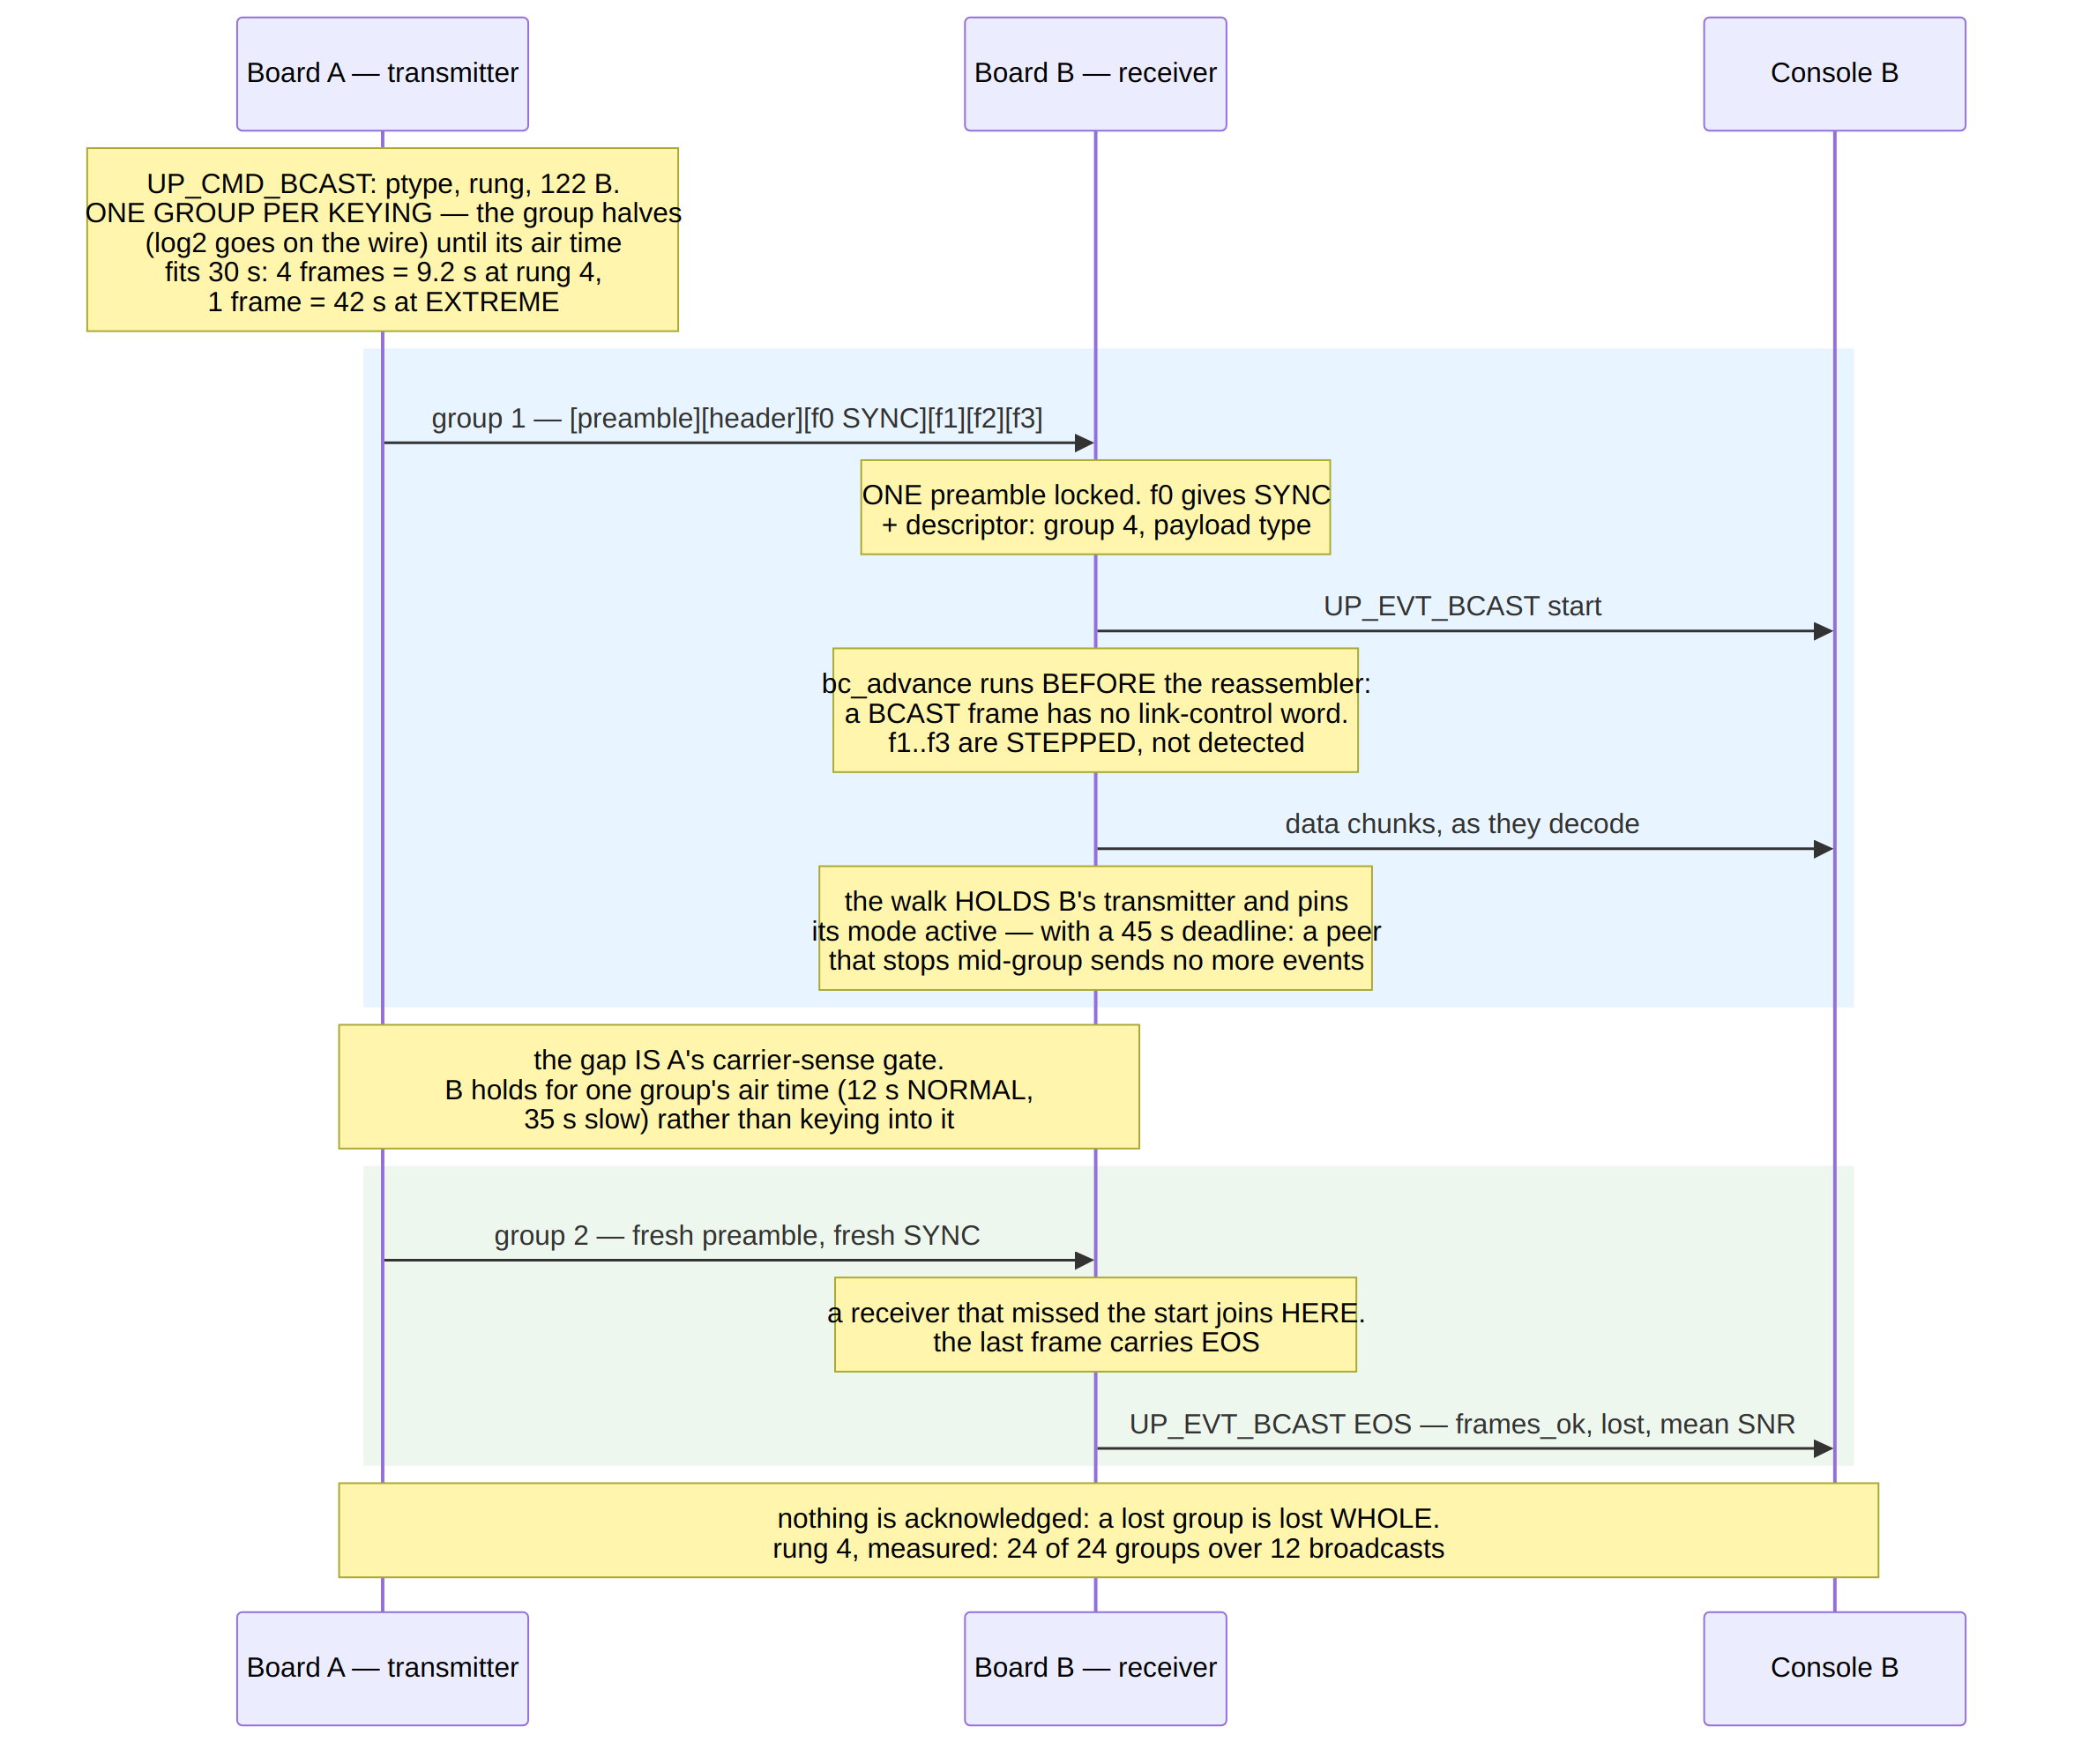
\includegraphics[width=0.85\textwidth]{images/bcast_boards.png}
    \caption{One broadcast between the two boards. The transmitter
             keys one group at a time; the receiver locks a single
             preamble per group, reads the descriptor from the SYNC
             frame and then \emph{steps} the remaining blocks without
             detecting again --- holding its own transmitter while it
             does. Nothing is acknowledged; until the block statistics
             of \S\ref{sec:bcstats}, the EOS frame's statistics were
             the entire feedback path.}
    \label{fig:bcastboards}
\end{figure}

\paragraph{The dispatch order is load-bearing.} A BCAST frame is
Data-shaped --- same header, same CRC, same block geometry --- but its
reserved field is not a link-control word. \texttt{bc\_advance()}
therefore runs \emph{before} \texttt{burst\_advance()} and the
station's reassembler; a broadcast frame reaching the latter would be
read as an ARQ fragment with a garbage sequence number and a garbage
acknowledgment request.

\paragraph{A walk that holds the transmitter must be able to expire.}
While the walk runs, the receiver is not running its detector at all
--- it is stepping to known block boundaries --- so the walk pins its
receiver instance active (muting one stops detection, and unmuting
rearms the search rather than resuming it) and gates the station's
key-up, for the reason Section~\ref{sec:cport_burstdebug} measured:
answering over a peer's live stream costs the rest of it. That leaves
the failure the burst walk already had to solve. The walk advances only
on events, and a peer that stops mid-group produces none: without a
deadline the board stays mute for good. With one --- 45\,s, a group's
air-time cap plus margin --- it recovers on its own.

\paragraph{One group is one keying.} Its air time is therefore bound
like everything else the station emits, and for the same reason the
224-second frames of Section~\ref{sec:cport_harden} were fatal. The
group size \emph{halves} --- $\log_2(\text{group})$ is what travels in
the SYNC descriptor, so it must stay a power of two --- until the group
fits 30\,s: four 26-byte frames are 9.2\,s at rung~4, while at EXTREME
a single frame is already 42\,s. The yield between groups is the
carrier-sense gate itself, and a station that has heard broadcast
traffic recently holds its own transmitter for about one group's worth
of time (12\,s at NORMAL, 35\,s at the slow modes) rather than keying
into the gap.

\subsubsection{The rung decides who can hear it}

A broadcast has no peer to negotiate with, which makes the rung a
choice rather than a measurement --- and the choice decides whether
anyone is listening at all. Which modes a board keeps active follows
the rung it has negotiated, and decays to EXTREME alone after a couple
of minutes of silence (Section~\ref{sec:cport_radio}); a broadcast sent
at a mode the intended listener has already dropped is inaudible, at
any signal level.

The first default got this wrong, and the wire said so within two
commands. It took \texttt{stats.last\_rung} --- what this station last
\emph{transmitted} at --- and floored it at rung~4 on the reasoning
that leaving the rung unspecified cannot mean ``take four minutes''.
On a link running at EXTREME that floor turns ``this link is at
EXTREME'' into ``broadcast at NORMAL'': the sending board keyed a
perfectly good NORMAL group, and the receiving board, whose ladder had
decayed to EXTREME-only listening, recorded a carrier at
$1.1\times10^{8}$ of mean square --- full strength --- with zero
capture drops, zero events and nothing decoded. Twice, with every
counter on both boards healthy.

The default is now the rung this station would send the peer an
ordinary frame at (\texttt{station\_tx\_rung()}: the controller's
answer, passed through the operator's ceiling and the peer's declared
maximum of \S\ref{sec:cport_caps}), which \emph{is} the peer's own
request and therefore the one rung the peer is certainly receiving
on. Nothing is floored --- a broadcast nobody can hear is worse than a
slow one, and the air-time cap keeps the slow case honest by collapsing
the group to a single frame. An explicit \texttt{-r} is still honoured
exactly as given, which is how a beacon reaches stations that have
never been heard from: EXTREME is the only mode an idle receiver is
guaranteed to have kept. And because ``nothing arrived'' looks
identical from the host whatever the cause, the board now logs the rung
it chose:

\begin{quote}\ttfamily\small
board: broadcast: 12 B at rung 0 (EXTREME), 1 frame(s) per group,
42.1 s each
\end{quote}

The measurements bracket both cases. A board freshly booted and having
never exchanged a frame --- listening on EXTREME alone --- received a
\texttt{bcast -r 0} byte-exact at $+16.2$\,dB, in two groups of one
frame each; the same transfer over a link \emph{running} at EXTREME,
which the floor used to break, now goes out at rung~0 and arrives. At
rung~4 with a 122-byte payload (two groups per broadcast, four frames
then two), a twelve-broadcast run delivered \textbf{24 of 24 groups},
72 frames, and reported zero losses at $+24.7$\,dB; across the whole
campaign 38 of 39 groups arrived.

\subsubsection{A file over the broadcast}

\texttt{bcastfile [-r <rung>] <path>} carries a file the same way ---
raw bytes, the opaque payload type, no delivery guarantee --- and the
receivers on every path (both consoles and the socket demo) store it
as \texttt{rx\_broadcast.bin}. The constraint worth the paragraph is
memory: the socket demo holds a 64\,kB source buffer because a PC
can, while the board's broadcast source is 8\,kB of DTCM, so the file
\emph{streams} from the host. Two bits of the command's payload-type
byte do the framing --- \emph{more follows} and \emph{continuation}
--- with both clear meaning the old one-shot broadcast, so nothing
existing changed; the host paces its chunks against a
\texttt{bc\_free} field the status frame now reports.

Chunking put two rules into the transmitter that the one-shot case
never needed. The EOS flag is emitted only once the host has declared
the stream complete --- an EOS computed from ``buffer drained'' would
fire at every pacing stall. And while chunks are still arriving, only
\emph{full} groups are keyed: a starved tail group would go out
without EOS, and the receiver's walk would never see the end of a
stream whose true last frame was still in transit over USB.

The first live run earned its regression comment. The C console's
chunk pump marked completion by setting its offset to $-1$ --- and
kept looping, because $-1$ is less than the length and the loop had no
\texttt{break}: it re-sent overlapping chunks twenty-four times, and
the receiving board stored 19\,380 bytes from a 1\,024-byte source.
(The Python console's pump, written the same hour, had the
\texttt{break}.) With the loop fixed and the board taught to ignore a
continuation when no broadcast is in flight, the retest delivered the
1\,kB file byte-exact in 19 seconds at rung~12 --- 44 frames in
eleven groups, zero lost, one completion message.

\paragraph{The negotiation belongs where the payload waits.} The
socket demo has always \emph{held} a broadcast on an idle link and
driven the ladder up first (\texttt{bc\_poll\_link}: control-class
probes every 25\,s, release when the link can carry a broadcast, give
up after 180\,s). Porting broadcast to the firmware left that
machinery host-side, on the reasoning that the host sees the status
stream and can probe with a message first --- and the first real
operator promptly typed \texttt{bcastfile} into two fresh consoles
and watched nothing happen, because the idle-link default is rung~0
and the first 42-second EXTREME frame shows no evidence of itself. Two
patches told the story in order: first the board's announce line
gained the \emph{consequence} (\texttt{$\sim$32 min total -- idle
link defaults to EXTREME: exchange a message first, or use -r}), and
then the honest fix landed --- \texttt{bc\_poll\_link} runs on the
board now, semantics line for line. Measured with the operator's exact
flow, no priming, no flags:

\begin{quote}\ttfamily\small
12:11:38 board: broadcast: held -- link is idle, probing to bring it
up (release at NORMAL, give up after 180 s)\\
12:12:14 board: broadcast: 1024 B at rung 12 (NORMAL), 4 frame(s) per
group, 1.6 s each, $\sim$18 s total\\
12:12:33 [B] stored 1024 bytes as rx\_broadcast.bin
\end{quote}

Thirty-six seconds from command to release, zero operator steps, the
LINK probe visible on the peer's console as an ordinary message. An
explicit \texttt{-r} bypasses the hold: the operator said where.

\paragraph{And the console needs no buffer at all.} The first
\texttt{bcastfile} read the whole file into a host buffer whose
64\,kB cap refused the first real file (a 73\,kB PNG). The cap was a
leftover of one-shot thinking: the pump is chunked and paced against
\texttt{bc\_free} anyway, so it now reads the file
\emph{sequentially}, a kilobyte per chunk as the board drains --- no
buffer, no cap, with a short read mid-stream (the file truncated
underneath the console) ending the broadcast cleanly rather than
leaving the board waiting for continuations forever. The board never
held more than its 8\,kB source either way; only the host had
forgotten that. Figure~\ref{fig:bcastfileseq} draws the complete
file-broadcast flow as it now stands --- the chunked feed, the hold
with the capability exchange as its probe, and the loss accounting the
campaign forced into the EOS statistics.

\begin{figure}[htbp]
    \centering
    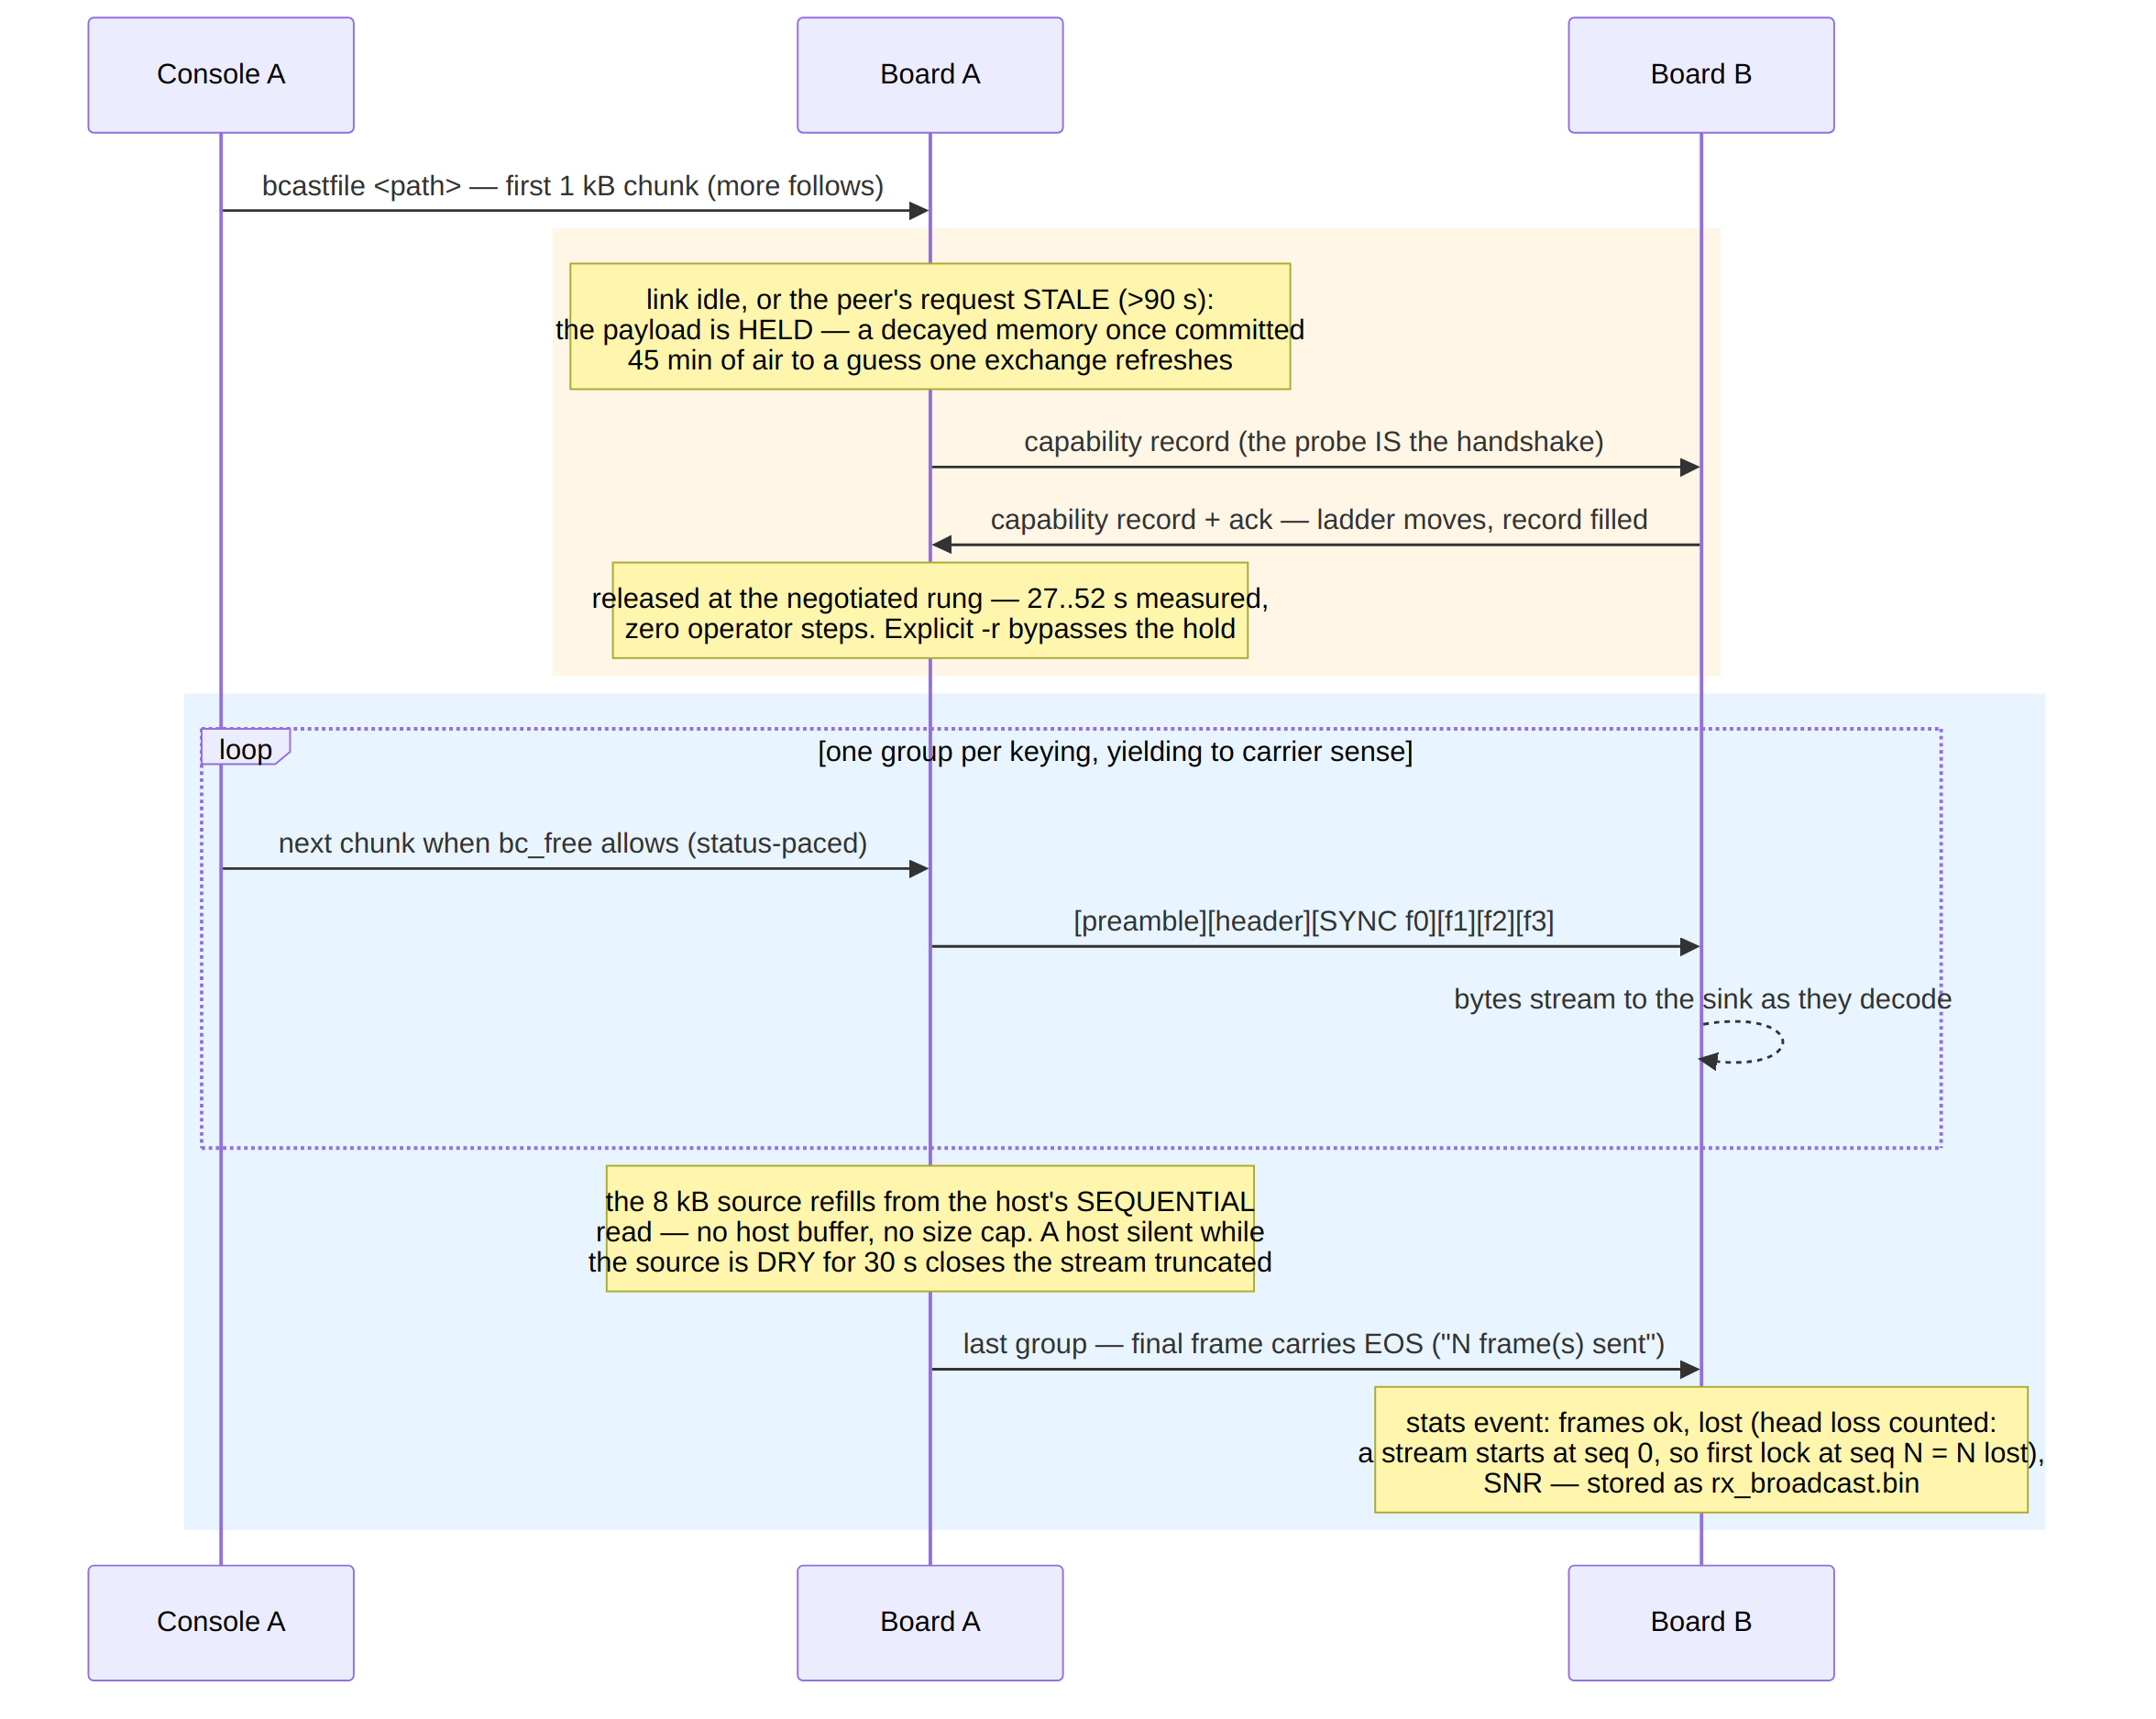
\includegraphics[width=0.72\textwidth]{images/bcastfile_seq.png}
    \caption{The chunk-fed file broadcast, end to end. The hold phase
             (top) probes with the capability record itself when the
             peer is a stranger --- or whenever the remembered rung has
             gone stale, after a 10-minute-old memory committed
             45~minutes of air to what one exchange refreshes. The
             stream phase repeats one group per keying, the host
             re-reading the file sequentially against the pacing field
             in the status stream.}
    \label{fig:bcastfileseq}
\end{figure}

Three stream-boundary rules came out of the file runs, each from a
measured failure.  An incomplete stream that a new command supersedes,
or whose host stops feeding, is closed on the air with a zero-length
EOS frame --- without one the stale tail of the aborted stream landed
in the next receiver's sink (a 73\,kB file arrived as 74\,027 bytes,
the first 665 belonging to the previous run).  The host-gone timeout
counts from the source running \emph{dry}, never from chunk gaps: at
rung~8 the drain is 38\,B/s and a healthy host's next chunk is
$\sim$27\,s out, so gap timing fired ``host stopped feeding'' three
times into a live transfer.  And the start event to the host fires
once per \emph{stream}, not per group, so consoles reset their sink on
every start they see.  The clean-run reference with all three in
place: 73\,362 bytes in 22.3\,min at rung~12, 3089 frames, 0 lost,
one start event, byte-identical.

\subsubsection{Blocks, receiver statistics, and a broadcast that
adapts}
\label{sec:bcstats}

The last extension makes the one-way street report back. When the
sender \emph{holds} a capability record whose new
\texttt{CAP\_BC\_STATS} bit is set --- the receiver's declaration
that it will answer, exactly the negotiation the operator asked for
--- the stream is cut into $\sim$45\,s blocks. Each block ends with
an \emph{end-of-block marker}: a dataless single-frame group (SYNC
flag, zero data bytes, no EOS), chosen over new frame flags because an
old receiver appends zero bytes for it and walks past --- the wire
stays compatible with every earlier firmware. The sender then pauses,
and the receiver answers with a small unicast frame (the last free
packet type): frames decoded, frames lost since the stream began, the
SNR, and the rung it wants. The sender logs the quality and
\emph{re-rungs the remaining groups}, which this wire has always
permitted --- every group re-announces its geometry in its SYNC
descriptor. Figure~\ref{fig:bcaststatsseq} traces the measured
exchange.

\begin{figure}[htbp]
    \centering
    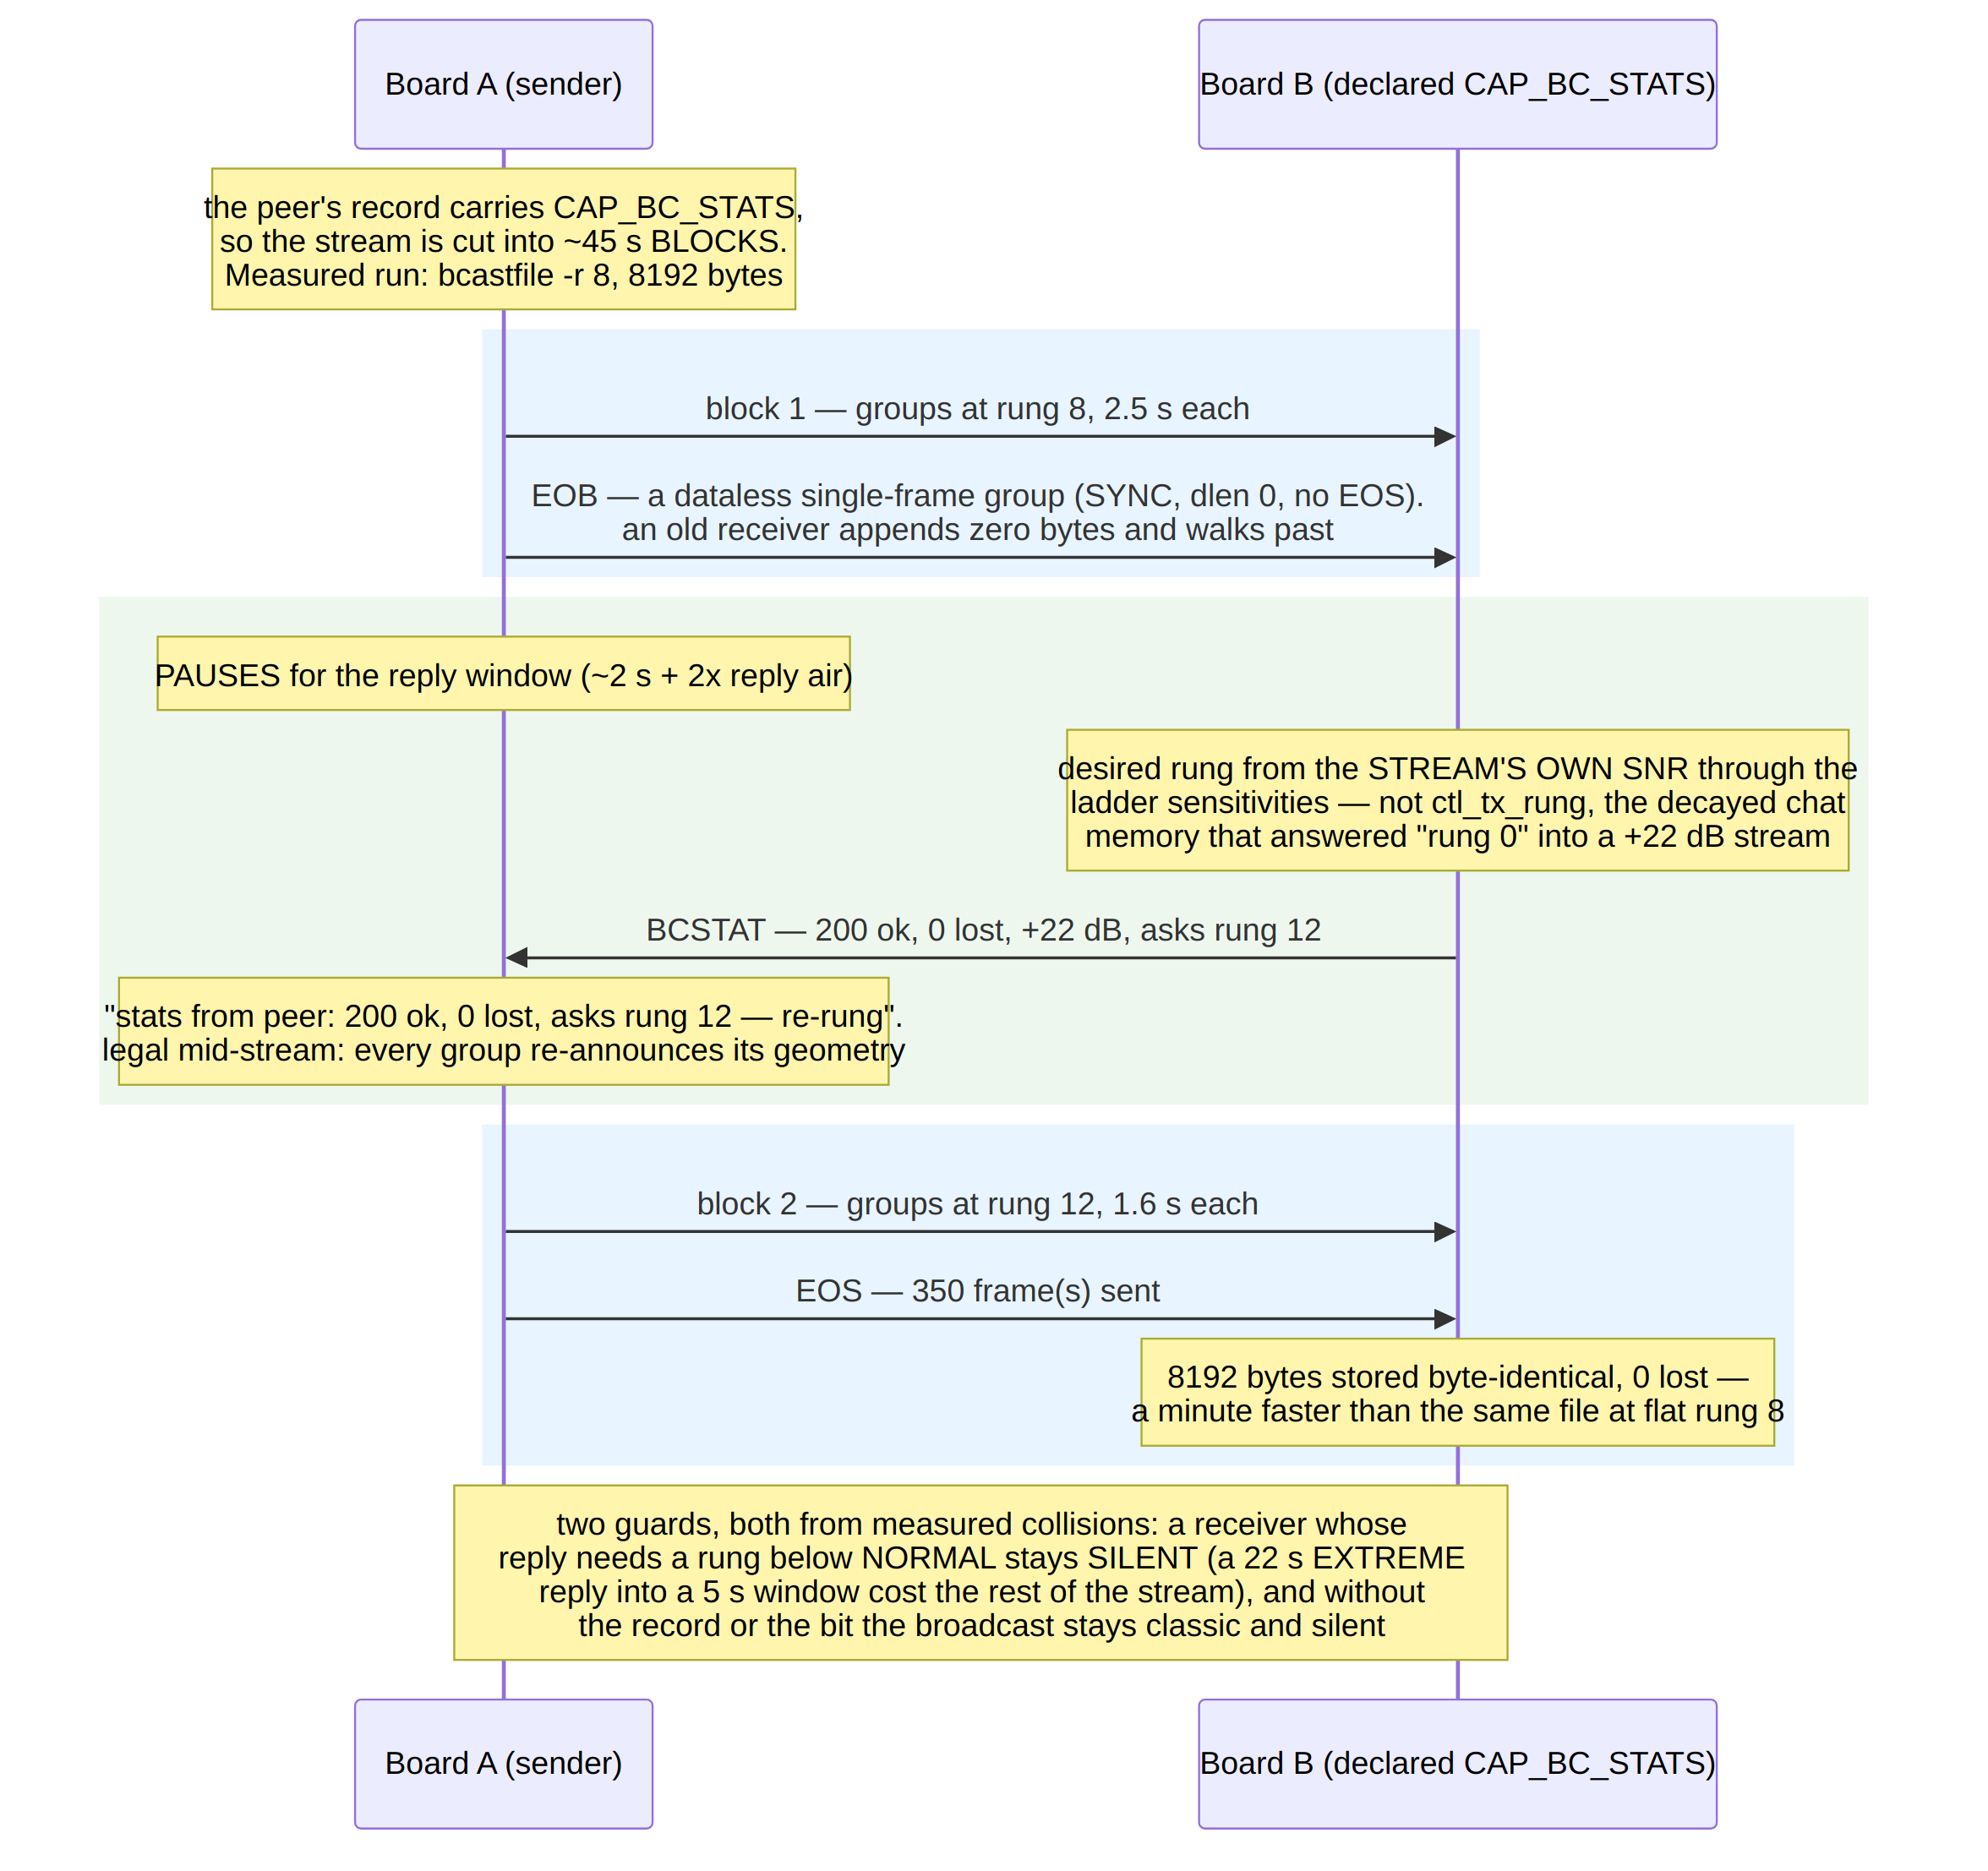
\includegraphics[width=0.66\textwidth]{images/bcast_stats_seq.png}
    \caption{Block statistics and the mid-stream re-rung, with the
             measured run's numbers. Both guard rules at the bottom
             came from collisions the first live runs produced.}
    \label{fig:bcaststatsseq}
\end{figure}

The first two live runs each contributed a rule. The receiver's
``desired rung'' initially came from its rate controller --- which is
the \emph{chat link's} decayed memory, and answered ``rung~0'' into a
stream it was decoding at $+22$\,dB; the request now comes from the
stream's own measured SNR mapped through the ladder sensitivities,
which is the question actually being asked. And the reply must
\emph{fit the window}: the first exchange keyed a 22-second EXTREME
stats frame into a five-second pause, the sender resumed its groups
mid-reply, and the collision cost the receiver the rest of the stream
--- 497 bytes stored of 8192. A receiver whose reply would need a rung
below NORMAL now stays silent, and silence is itself information.

The verification run started deliberately slow: \texttt{bcastfile -r
8}, 8192 bytes. One block later the stats frame came back --- \texttt{200
ok, 0 lost, asks rung 12 -- re-rung} --- the remaining groups went out
at rung~12, and the file stored byte-identical with 350 frames and
zero lost, a minute faster than the same file at flat rung~8. A
broadcast to strangers, or to a peer that never declared the bit,
remains exactly the classic silent stream.

\subsubsection{Adaptation under a fade}
\label{sec:bcfade}

The wire between the boards cannot fade, so the fading test is a host
twin in the project's usual style: \texttt{make bcfade} runs the
firmware's block/stats/re-rung machinery --- sender state machine,
receiver walk, both control decisions --- over an AWGN channel whose
SNR follows a V-shaped profile ($+20 \to -5 \to +20$\,dB over a
60-second floor). Its first run earned the harness its place: the
adaptation \emph{did not adapt}. The receiver's SNR estimate is
measured only on frames strong enough to decode --- survivorship bias
--- and read $+22$\,dB inside the $-5$\,dB fade while 41\% of a
block died; meanwhile the EOB markers and stats replies died with the
fade, so the feedback vanished exactly when it was needed. Two control
laws fix it, harness-proven and then ported to the firmware verbatim:
a lossy block anchors its rung request on the receiver's \emph{own
last ask}, never on the SNR, with severe loss ($>$40\%) going
straight to the NORMAL floor; and a promised reply that never arrives
steps the sender down two rungs and shortens the next block to 20\,s
--- silence is itself feedback. On identical fades:

\begin{center}
\begin{tabular}{llcl}
\hline
fade floor & arm & delivered (of 8192) & rung trajectory \\
\hline
$-5$\,dB & fixed rung 12 & 4154 & 12 throughout \\
$-5$\,dB & adaptive & \textbf{5481 ($+32$\%)} & $12 \to 10 \to 8 \to 4 \to 12$ \\
$-2$\,dB & fixed rung 12 & 4392 & \\
$-2$\,dB & adaptive & \textbf{6100 ($+39$\%)} & \\
\hline
\end{tabular}
\end{center}

Figure~\ref{fig:bcastfadeseq} draws the measured deep-fade run as the
exchange the two ends actually had --- including the two windows in
which nothing was exchanged at all, which is where half the control
law lives.

\begin{figure}[t]
    \centering
    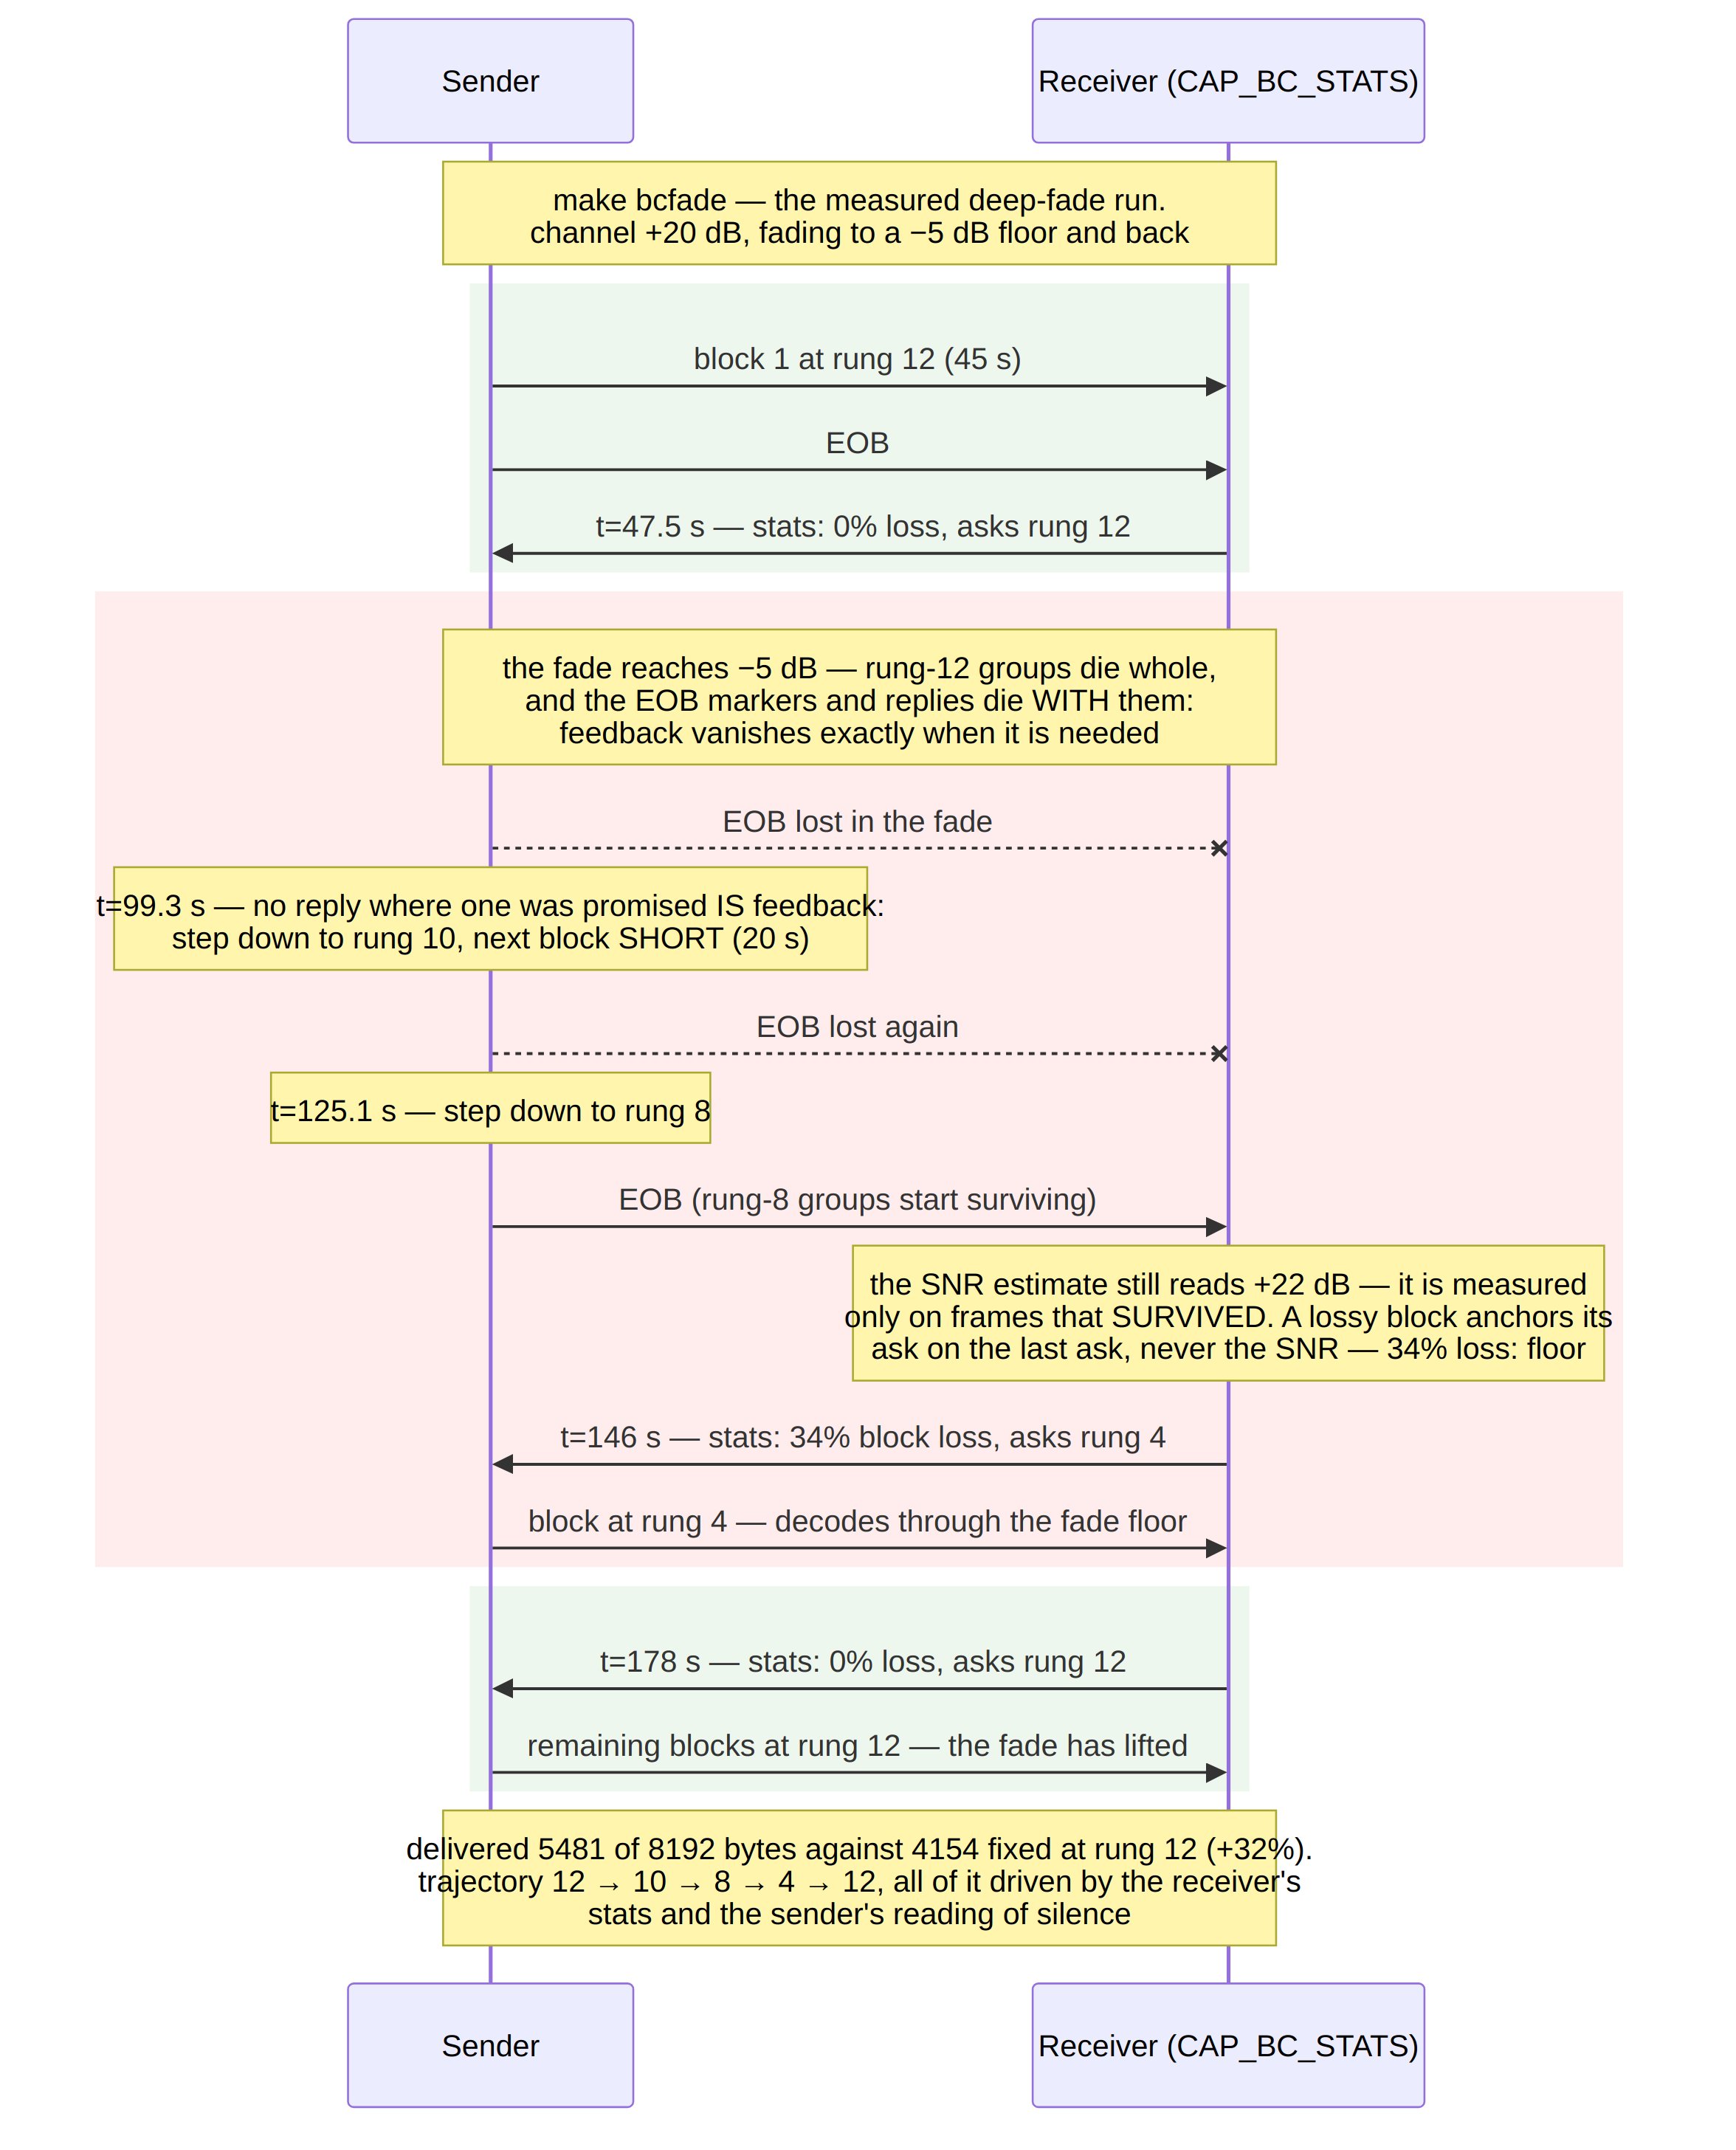
\includegraphics[width=0.52\textwidth]{images/bcast_fade_seq.png}
    \caption{The deep-fade run of \texttt{make bcfade}, drawn from its
             transcript. The red span is the $-5$\,dB floor: the lost
             EOB markers become step-downs (silence as feedback), the
             survivorship-biased SNR is overruled by the block's loss
             rate, and the rung-4 blocks carry the stream through the
             floor until the recovery ask lifts it back.}
    \label{fig:bcastfadeseq}
\end{figure}
